\subsection{Set Covering Problem}
\subsubsection{SCP formulation}
The SCP is a well-known mathematical problem, which tries to cover a set of needs at the lowest possible cost. The SCP was included in the list of 21  $\mathcal{N} \mathcal{P}$-\textit{complet} problems of Karp \cite{DBLP:books/daglib/p/Karp10}. There are many practical uses for this problem, such as: crew scheduling \cite{ref02, ref08}, location of emergency facilities \cite{ref51,Vasko198485}, production planning in industry \cite{Vasko:1987:OSI:40299.40301,ref48, ref50}, vehicle routing \cite{ref07, ref27}, ship scheduling \cite{ref26, ref13}, network attack or defense \cite{ref14}, assembly line balancing \cite{ref28, ref41}, traffic assignment in satellite communication systems \cite{ref37, ceriaetal1998}, simplifying boolean expressions \cite{ref16}, the calculation of bounds in integer programs \cite{ref18}, information retrieval \cite{ref20}, political districting \cite{ref29}, crew scheduling problems in airlines \cite{doi:10.1287/inte.27.5.68}, among others.
The SCP can be formulated as follows:

\begin{equation} \label{ec:set-covering-1}  
\mbox{Minimize} \quad Z = \sum_{j = 1}^{n} c_j x_j
\end{equation}
Subject to:
\begin{equation} \label{ec:set-covering-2} 
\sum_{j = 1}^{n} a_{ij} x_j \geq 1 \quad  \forall i \in I
\end{equation}
\begin{equation} \label{ec:set-covering-3} 
x_j \in \{0,1\} \quad  \forall j \in J 
\end{equation}	


Let $A = (a_{ij})$ be a $m \times n$ 0-1 matrix with $I = \{ 1,\dots, m\}$ and $J = \{ 1,\dots, n\}$ be the row and column sets respectively. We say that column $j$ can be cover a row $i$ if $a_{ij} = 1$. Where $c_j$ is a nonnegative value that represents the cost of selecting the column $j$ and $x_j$ is a decision variable, it can be 1 if column $j$ is selected or 0 otherwise. The objective is to find a minimum cost subset $S \subseteq J$, such that each row $i \in I$ is covered by at least one column $j \in S$. 
\vspace{0mm}\\

In the following section, we present a simple way to understand the SCP, through an example:\\

\subsubsection{SCP sample solution}
Imagine that an ambulance station can meet the needs of an geographic zone. Similarly the ambulance station can cover all the needs of the nearby areas. For example, if a station is built in Zone 1 (Figure~\ref{fig:SetCovering}) ambulance station can meet the needs of neighboring areas, that is, it could also cover: Zone 1, Zone 2, Zone 3 and Zone 4.  This can be appreciated in equation (\ref{ec:rest1}).

In this example, we must fulfill the need to cover the geographical areas defined in accordance with the restrictions.

The restriction of this case is that all areas must be covered by at least one ambulance station and the goal is to minimize the number of stations built, the cost of building a station is the same for all areas. The $x_j$ variable represents the area $j$ which is $1$ if the ambulance station is built, and will be $0$ if not. As above, it can be formulated as follows:

\squeezeup
\begin{figure}[!http]
	\begin{center}
		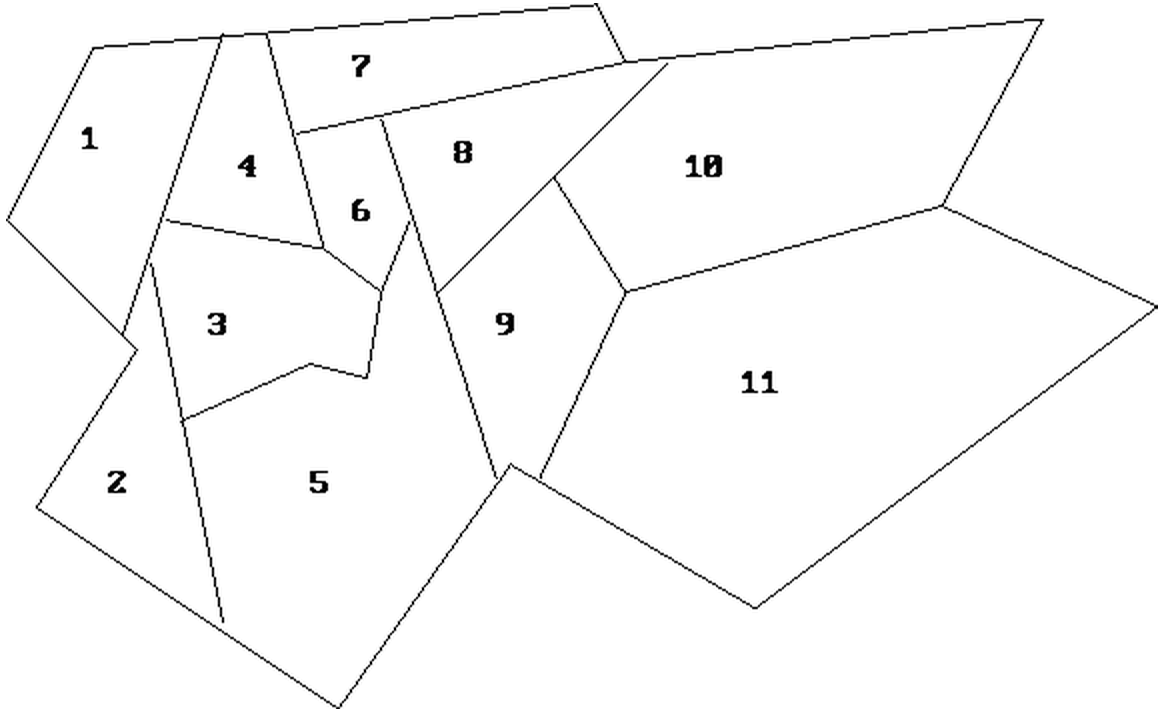
\includegraphics[width=0.5\linewidth]{Introduccion/imagenes/SetCovering.png}
		\caption{Set Covering Problem example.}\label{fig:SetCovering}
	\end{center}
\end{figure}
\squeezeup


\scriptsize
\begin{equation} \label{ec:SetCoveringExample} 
\mbox{Min} \quad c_{1}x_{1} + c_{2}x_{2} + c_{3}x_{3} + c_{4}x_{4} + c_{5}x_{5} + c_{6}x_{6} + c_{7}x_{7} + c_{8}x_{8} + c_{9}x_{9} + c_{10}x_{10} + c_{11}x_{11}
\end{equation}

Subject to:
\begin{align}
x_{1} & + & x_{2} & + & x_{3} & + & x_{4} &  &  &  &  &  &  &  &  &  &  &  &  &  &  & \geq  1 \label{ec:rest1}  \\
x_{1} & + & x_{2} & + & x_{3} &  &  & + & x_{5} &  &  &  &  &  &  &  &  &  &  &  &  & \geq  1 \\
x_{1} & + & x_{2} & + & x_{3} & + & x_{4} & + & x_{5} & + & x_{6} &  &  &  &  &  &  &  &  &  &  & \geq  1 \\
x_{1} &  &  & + & x_{3} & + & x_{4} &  &  & + & x_{6} & + & x_{7} &  &  &  &  &  &  &  &  & \geq  1 \\
& & x_{2} & + & x_{3} &  &  & + & x_{5} & + & x_{6} &  &  & + & x_{8} & + & x_{9} &  &  &  &  & \geq  1 \\
& & & & x_{3} & + & x_{4} & + & x_{5} & + & x_{6} & + & x_{7} & + & x_{8} &  &  &  &  &  &  & \geq  1 \\
& & & & & & x_{4} & & & + & x_{6} & + & x_{7} & + & x_{8} & & & & & & & \geq  1 \\
& & & & & & & & x_{5} & + & x_{6} & + & x_{7} & + & x_{8} & + & x_{9} & + & x_{10} & & & \geq  1 \\
& & & & & & & & x_{5} & & & & & + & x_{8} & + & x_{9} & + & x_{10} & + & x_{11} & \geq  1 \\
& & & & & & & & & & & & & & x_{8} & + & x_{9} & + & x_{10} & + & x_{11} & \geq  1 \\
& & & & & & & & & & & & & & & & x_{9} & + & x_{10} & + & x_{11} & \geq  1 
\end{align}
\normalsize

The first constraint (\ref{ec:rest1}) indicates that to cover zone 1, it is possible to locate a station in the same area or in the border. The following restriction is for zone 2 and so on. One possible optimal solution for this problem is to locate ambulance stations in zones 3, 8 and 9. That is, $x_{3} = x_8 = x_9 = 1$ y $x_{1} = x_{2} = x_{4} = x_{5} = x_{6} = x_{7} = x_{10} = x_{11} = 0$. As shown in (Figure~\ref{fig:SetCovering2}).

\squeezeup
\begin{figure}[!http]
	\begin{center}
		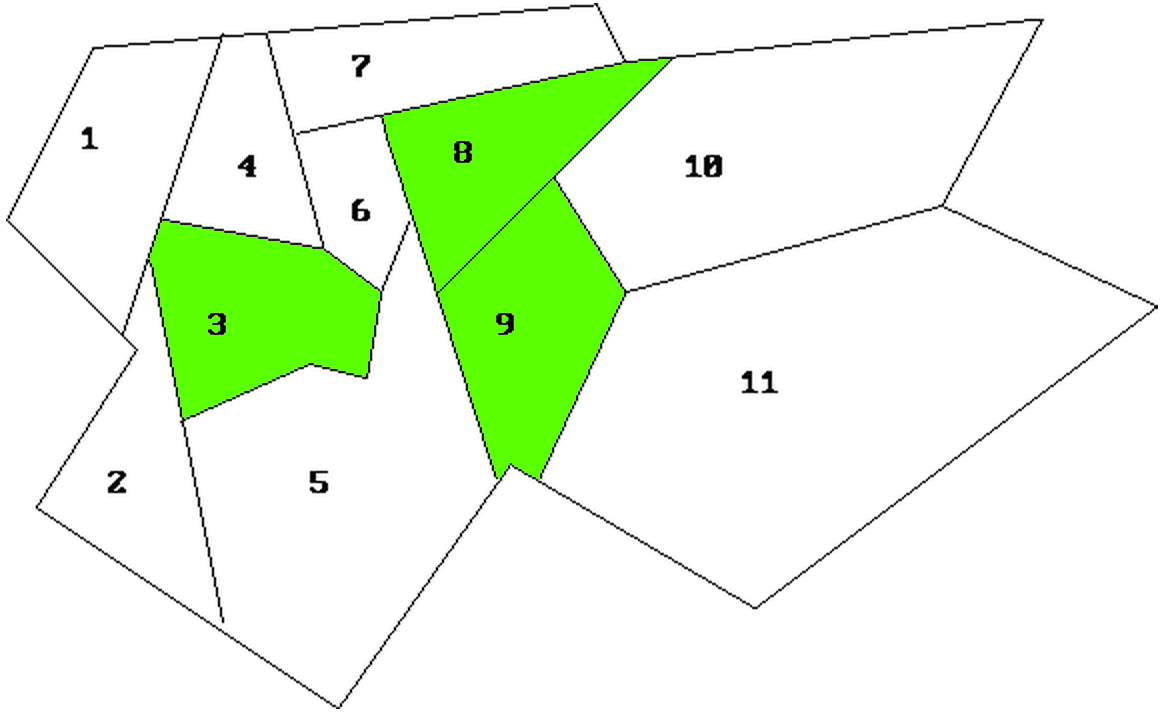
\includegraphics[width=0.5\linewidth]{Introduccion/imagenes/SetCoveringSolved.png}
		\caption{Set Covering Problem solution.}\label{fig:SetCovering2}
	\end{center}	
\end{figure}
\squeezeup

%\subsection{Unicost SCP}
%The Unicost \cite{DBLP:conf/ieaaie/Musliu06,DBLP:journals/eor/AzimiTG10} is a variation of the SCP where the cost of each decision variable is 1. This indicates that it does not matter which one is active, what matters is to comply with the restrictions.


We propose solve the SCP, with a variation metaheuristic Harmony Search (HS) called Binary Global-Best Harmony Search to obtain satisfactory solutions within a reasonable time. HS mimics the process of musical improvisation, where musicians make adjustments in tone to achieve aesthetic harmony.